\section{Preliminaries: Continuous-Time Markov Chains and Masked Diffusions}
\label{sec:pre}
In what follows, we provide an overview of continuous-time Markov chains (CTMCs), their role in defining discrete diffusion models, and link them to the MDM framework. As we mentioned in the introduction, this theme is essential to defining FlexMDMs in Section~\ref{sec:FlexMDM_informal}.

\textbf{Transport with continuous-time Markov Chains.} Given a target distribution $p_1$ over sequences with a finite vocabulary set (e.g., text), our aim is to learn to transport samples from a reference distribution $p_0$ through a continuum of distributions $\{p_t\}_{t \in [0,1]}$ such that $p_{t=1} = p_1$. This type of transport can be realized by a continuous-time Markov chain, which is a stochastic process $\{X_t\}_{t\in[0,1]}$ with $X_0 \sim p_0$ governed by a time-dependent transition rate matrix  $\{R_t(\cdot,\cdot)\}_{t\in[0,1]}$ satisfying
\begin{equation} \label{eq:mass-conservation}
    R_t(x, x)= -\sum_{y \neq x} R_t(x, y), \quad R_t(x,y) \ge 0,\,\, x \ne y.
\end{equation}
Intuitively, the rate matrix determines the infinitesimal likelihood that $X_t$ transitions to any other state $y$ via 
%
\begin{equation} \label{eq:transition}
    \mathbb P(X_{t+h} = y | X_t = x) = \mathbf{1}_{\{x = y\}} + h R_t(x,y) + o(h)\,,
\end{equation}
%
where we denote the conditional probability measure $\mathbb P(\cdot |X_{t} = x)$ of a new state given the present one. Here $o(h)$ is a remainder term that vanishes faster than $h$ as $h\rightarrow 0$. 
In generative modeling for these discrete distributions, our aims are to \textbf{(a)} specify a path of marginal distributions $\{p_t\}_{t\in[0,1]}$ connecting $p_0$ to $p_1$ and \textbf{(b)} learn the associated $R_t$ such that these marginals collectively satisfy the Kolmogorov forward equation:
%
\begin{equation} \label{eq:kfe}
\partial_t p_t(x) = \sum_y p_t(y) R_t(y, x)  \qquad p_{t=0} = p_0.
\end{equation}
%
This ensures that at time $t = 1$, the evolution specified by~\eqref{eq:transition} results in a sample from the target distribution $p_1$. The rate matrices defined in this paper are sparse; therefore, we assume that the unspecified entries are $0$ and the diagonal entries are defined through Equation~\eqref{eq:mass-conservation}.
\subsection{Masked Diffusion Models}
 We briefly review MDMs~\citep{sahoo2024simple,shi2024simplified} and discrete flow matching with the masked construction ~\citep{gat2024discrete}, through the lens of stochastic interpolants. The target distribution $p_1$ assigns probability to length $L$ sequences. The base distribution $p_0$ employed by these models is the point mass distribution at the fully masked length-$L$ sequence $(\mask, \dots, \mask)$, where $\mask$ is an auxiliary mask token. 

To define the intermediate $\{p_t\}_{t \in [0,1]}$ that bridges the base and the target, we make use of a \coloredhl{xblue}{stochastic interpolant} $\{x_t\}_{t\in[0,1]}$, a collection of random variables whose marginal distribution defines the continuum $\{p_t\}_{t\in[0,1]}$, i.e., $x_t \sim p_t$. Although the previous notion of stochastic interpolant~\citep{albergo2023stochastic} is defined in a continuous space, it naturally extends to a discrete space, and we defer a formal exposition to Appendix~\ref{sec:appendix_theory_interpolant}.

\begin{minipage}{0.52\textwidth}
\textbf{Design of distribution path.} The stochastic interpolant relies on a smooth and monotone unmasking schedule $\alpha_t \colon [0,1]\to [0,1]$ with boundary condition $(\alpha_0,\alpha_1)=(0,1)$ and time derivative denoted by $\dot{\alpha_t}$. 
To draw $x_t$, we first sample a clean sequence $x_1 \sim p_1$; then, independently for every coordinate $i$, we draw an unmasking time $T^i$ from density $\dot{\alpha}_tdt$ and set 
\begin{equation*}
    x_t^i\, =\, \begin{cases}
        \mask & t < T^i\\
        x_1^i & t \ge T^i
    \end{cases}.
\end{equation*}
This process is illustrated in Figure~\ref{fig:interpolant_mdm}. Hence, each clean token stays masked with probability $1 - \alpha_t$ in a coordinate-independent fashion, defining $p_t(\cdot \mid x_1)$. We then write $p_t$ by marginalizing over $x_1\sim p_1$.
\end{minipage}
\hfill
\begin{minipage}{0.46\textwidth}
\begin{figure}[H]
\centering
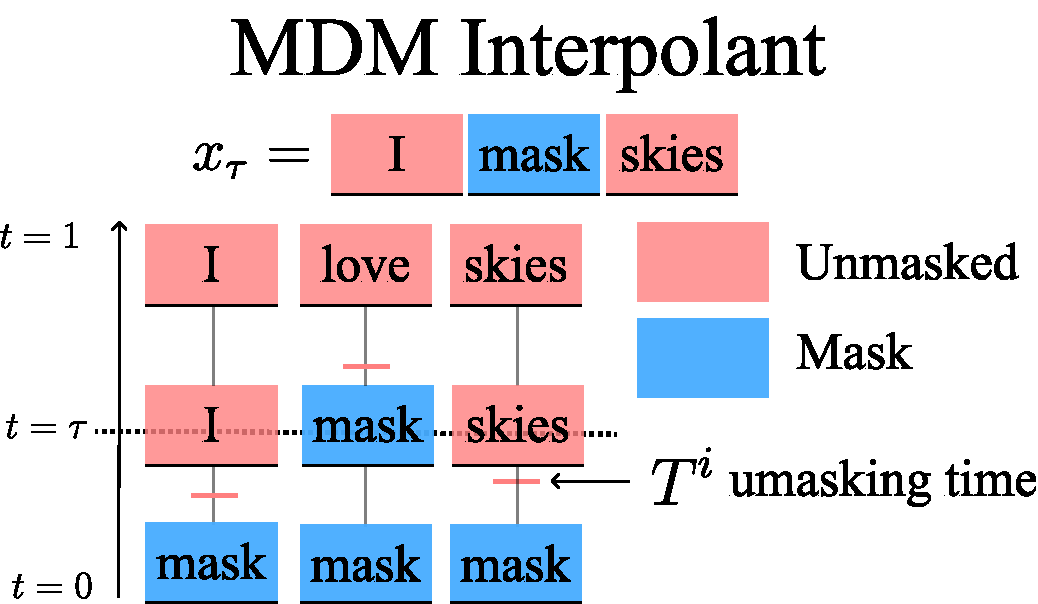
\includegraphics[width=\textwidth,trim={0 0 0 2.0cm}]{Figures/mdm_new.pdf}
\caption[\textbf{MDM interpolant.}]{To draw a sample $x_t$, one can equivalently sample the clean sequence $x_1\sim p_1$, draw unmasking times, and then accordingly \coloredul{xred}{unmask} or \coloredul{xblue}{mask} each coordinate's token.}\label{fig:interpolant_mdm}
\end{figure}
\end{minipage}

\textbf{MDM training.} We now derive the MDM rate matrix that induces a CTMC whose marginals coincide with $\{p_t\}_{t\in[0,1]}$ and how it is learned in practice. The central object is the \coloredhl{xblue}{unmasking posterior}: the posterior on the clean token $x_1^i$ for masked index $i$ given $x_t=x$ and time step $t$, i.e., $\mathbb{P}(x_1^i = v | x_t = x)$. We model this posterior with a neural network $f_\theta(x,t) \in (\Delta(\Sigma))^n$, where $\Delta(\Sigma)$ denotes a simplex of probability distributions over the vocabulary $\Sigma$. 

For every position where $x^i=\mask$, the network aims to predict $f_\theta(x,t)[i,v]\approx \mathbb{P}(x_1^i = v | x_t = x)$,  and is trained by minimizing the following variational loss:
%
{\small
\begin{equation}
\label{eq:loss:mdm}
\mathcal{L}_\theta = -\int_{0}^1 \mathbb{E}\left[\frac{\dot{\alpha}_t}{1-\alpha_t}\sum_{i \colon x_t^i = \mask} \xblue{\log f_{\theta}(x_t, t)[i,x_1^i]} \right]dt.
\end{equation}}

Here, $\mathbb{E}$ denotes the expectation over $x_1 \sim p_1$ and $x_t\sim p_t(\cdot|x_1)$. The minimizer of this loss is the ground-truth unmasking posterior, which fully determines the MDM's rate matrix below. Precisely, for $t\in [0,1]$, the rate matrix at time $t$ is given by: for a partially masked sequence $x \in (\Sigma \cup \{\mask\})^L$,
\begin{equation} \label{eq:rate_mdm}
   R_t(x, \replaceat{x}{i}{v}) = \frac{\dot{\alpha_t}}{1-\alpha_t}\underbrace{\mathbb{P}(x_1^i = v | x_t = x)}_{\xblue{\text{unmasking posterior}}} , \quad  v \in \Sigma, x^i=\mask,
\end{equation}
where $\replaceat{x}{i}{v}$ denotes the sequence obtained from $x$ by replacing its $i$-th token with $v$. Therefore, once $f_\theta$ has learned the unmasking posterior, one can simulate the CTMC using the rate matrix in ~\eqref{eq:rate_mdm}. The variational loss \eqref{eq:loss:mdm} quantifies the sampling guarantee of this \emph{estimated} CTMC. Let $p_1^\theta$ be the terminal distribution of the estimated CTMC. Then, the loss function bounds the KL-divergence:
\begin{equation*}
    \mathcal{D}_{\mathrm{KL}}(p_1 || p_1^\theta) \leq \mathcal{L}_\theta - \mathcal{L}_\star,
\end{equation*}
where $\mathcal{L}_\star$ is the global minimum of $\mathcal{L}$. When the loss is in its infimum, the KL divergence vanishes, resulting in the ground truth distribution.

\textbf{Connections to other MDM frameworks.} Connecting to prior works on MDM ~\citep{shi2024simplified, sahoo2024simple, campbell2022continuous}, defining an interpolant is similar to defining a forward process for the case of diffusion models or a probability path in the case of flow matching. The modeled quantity is identical to the unmasking posterior across all frameworks. For inference, a common scheme is to proceed by: at each intermediate time step, (a) selecting a subset of indices to unmask and (b) sampling clean tokens from the learned posterior. In the infinitesimal limit, this procedure is equivalent to simulating the CTMC of \eqref{eq:rate_mdm}. Meanwhile, subsequent work \cite{kim2025train,nie2025large} shows that MDMs also allow theoretically grounded \emph{any-order inference}: tokens can be unmasked in an arbitrary order without necessarily following the CTMC at \eqref{eq:rate_mdm}. We will revisit this aspect in Section~\ref{sec:FlexMDM_inference} and show that our FlexMDM preserves this advantage.